\documentclass[12pt, dvipdfmx]{beamer}
%\documentclass[8,9,10,11,12,14,17,20pt, dvips, handout]{beamer}
%%%%%%%%%%%  package  %%%%%%%%%%%
\usepackage{amssymb,amsmath,ascmac}
\usepackage{atbegshi}
\AtBeginShipoutFirst{\special{pdf:tounicode 90ms-RKSJ-UCS2}}
\usepackage{minijs}
\renewcommand{\kanjifamilydefault}{\gtdefault}
\usepackage{multirow}

\usepackage[dvipdfmx]{animate}
\usepackage{graphicx}
\usepackage{bm}

%\usepackage{tikz}
%\usepackage{xparse}
%\usetikzlibrary{shapes,arrows}
%%% define fancy arrow. \tikzfancyarrow[<option>]{<text>}. ex: \tikzfancyarrow[fill=red!5]{hoge}
%  \tikzset{arrowstyle/.style n args={2}{inner ysep=0.1ex, inner xsep=0.5em, minimum height=2em, draw=#2, fill=black!20, font=\sffamily\bfseries, single arrow, single arrow head extend=0.4em, #1,}}
%  \NewDocumentCommand{\tikzfancyarrow}{O{fill=black!20} O{none}  m}{
%    \tikz[baseline=-0.5ex]\node [arrowstyle={#1}{#2}] {#3 \mathstrut};}

%%%%%%%%%%%  theme  %%%%%%%%%%%
\usetheme{Copenhagen}

%%%%%%%%%%%  inner theme  %%%%%%%%%%%
\useinnertheme{default}

%%%%%%%%%%%  outer theme  %%%%%%%%%%%
\useoutertheme{default}

%%%%%%%%%%%  font theme  %%%%%%%%%%%
\usefonttheme{professionalfonts}

%%%%%%%%%%%  degree of transparency  %%%%%%%%%%%
\setbeamertemplate{items}[default]

%%%%%%%%%%%  numbering  %%%%%%%%%%%
\setbeamertemplate{navigation symbols}{}

\title
[時空相関関数]
{時空相関関数について}
\author{佐々木裕}
\institute{東亞合成}
\date{\today}
\begin{document}

%%%%%
% 1 P
%%%%%
\begin{frame}\frametitle{}
	\titlepage
\end{frame}

\section{はじめに}


% %%%%%%%%%%%%%%%%%%%%%%%%%%
% \subsection{評価について}
% %%%%%%%%%%%%%%%%%%%%%%%%%%%

% %%%%%%%%%%%%%
% \begin{frame}
% \frametitle{評価について}

% \begin{itemize}
% \item
% 時空相関関数

% 	時空相関関数のセルフパート $G_s(\bm{r}, t)$ を算出し、その時間変化からクラスタ内のセグメントのダイナミクスを評価
% \end{itemize}

% \end{frame}
% %%%%%%%%%%%%

%%%%%%%%%%%%%
\begin{frame}
\frametitle{時空相関関数(あるいは、van Hove 関数)}
\vspace{-2mm}
\begin{columns}[T, totalwidth=\linewidth]
\column{.56\linewidth}
\begin{block}{時空相関関数 $G(\bm{r}, t)$ の定義}
\vspace{-4mm}
\scriptsize
\begin{equation*}
G(\bm{r}, t) = \dfrac{1}{N}\left\langle \sum_{i=1}^{N} \sum_{j=1}^{N} \delta[\bm{r} + \bm{r}_j(0) - \bm{r}_i(t)] \right\rangle
\end{equation*}
\normalsize
\end{block}
\vspace{-1mm}
\begin{block}{self part と distinct part}
\vspace{-4mm}
\scriptsize
\begin{align*}
	&G(\bm{r}, t) = G_s(\bm{r}, t) + G_d(\bm{r}, t) \\
	&\begin{cases}
	\text{自分自身との相関である self part:}\\
	G_s(\bm{r}, t) = \dfrac{1}{N}\left\langle \displaystyle \sum_{i=1}^{N} \delta[\bm{r} + \bm{r}_i(0) - \bm{r}_i(t)] \right\rangle \\[12pt]
	\text{異なる粒子間の相関だけの distinct part:}\\
	G_d(\bm{r}, t) = \dfrac{1}{N}\left\langle \displaystyle \sum_{i \neq j}^{N} \displaystyle \sum_{j=1}^{N} \delta[\bm{r} + \bm{r}_j(0) - \bm{r}_i(t)] \right\rangle
 	\end{cases}
\end{align*}
\normalsize
\end{block}

\column{.4\linewidth}
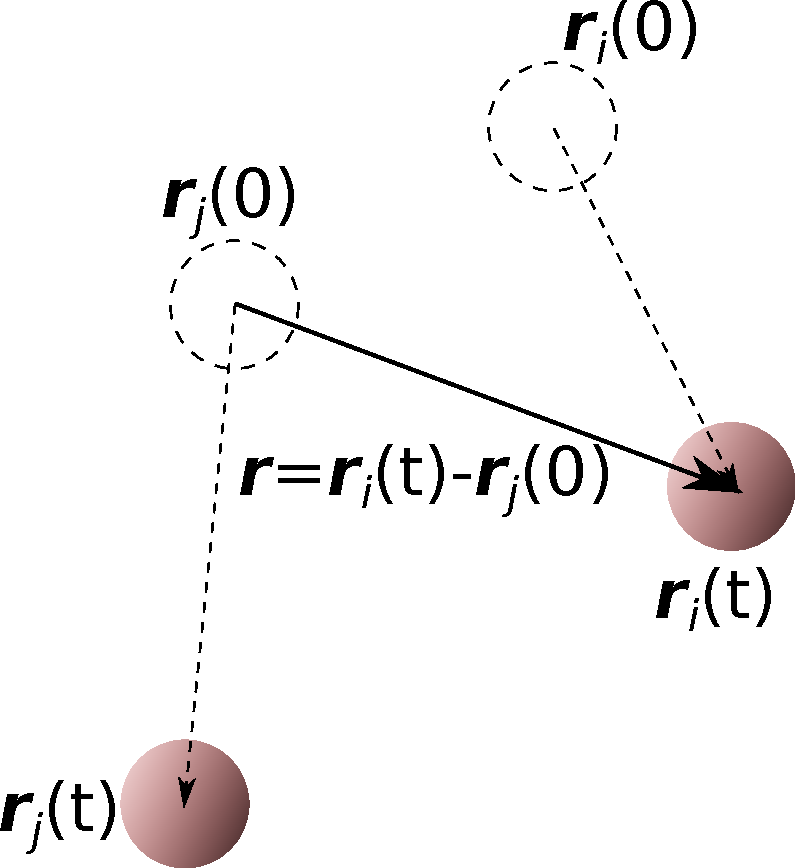
\includegraphics[width=\columnwidth]{G(rt).pdf}

\centering
粒子の移動のイメージ\\
$\bm{r}_i(0) \rightarrow \bm{r}_i(t)$ へと移動

\end{columns}
\end{frame}
%%%%%%%%%%%

%%%%%%%%%%
\begin{frame}
%[shrink squeeze]
%[allowframebreaks]
\frametitle{self part: $G_s(\bm{r}, t)$ によるクラスタの評価}

\begin{columns}[T, totalwidth=0.96\linewidth]
\column{.47\linewidth}

\begin{block}{$G_s(\bm{r}, t)$ の特性}
	\begin{itemize}
	\item
%	\footnotesize
	全空間で積分すれば 1\\
%	\scriptsize
%	\begin{equation*}
%	\int G_s(\bm{r}, t) {\rm d} \bm{r} = 1
%	\end{equation*}
%	\normalsize
	\item
%	\footnotesize
	$t=0$ で、デルタ関数
%	\scriptsize
%	\begin{equation*}
%	G_s(\bm{r}, 0) = \delta (\bm{r})
%	\end{equation*}
%	\normalsize
	\item
%	\footnotesize
	時間経過に伴う空間的な広がりを評価可能
	\end{itemize}
\end{block}

\begin{alertblock}{クラスタ内の評価}
%\footnotesize
クラスタ空間からのセグメント脱離の評価
\end{alertblock}

\column{.47\linewidth}
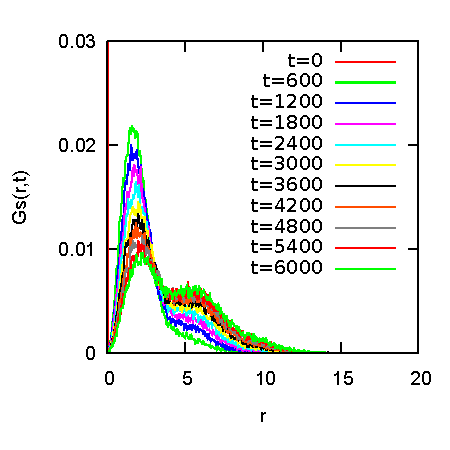
\includegraphics[width=\columnwidth]{Ave_Trj.pdf}

\centering
トリブロックコポリマーのクラスタ部に対する $G_s(\bm{r}, t)$ の例
\end{columns}
\end{frame}
%%%%%%%%%%%



%%%%%
\begin{frame}

\frametitle{クラスタからの脱離の評価}

\begin{columns}[T, totalwidth=\linewidth]
\column{.47\linewidth}
A セグメントの時空相関関数のセルフパート $G_s(\bm{r}, t)$ を評価した。

$t=0$ において $r=0$ に立っていた $\delta$ 関数が、時間の経過に伴い、{\color{red} 空間的になまされていく過程}が確認できる。

\begin{exampleblock}{脱離の評価}
$G_s(\bm{r}, t)$ をクラスタが占めるであろう空間領域で積分し、その時間変化をモニタする。
\end{exampleblock}

\column{.47\linewidth}

	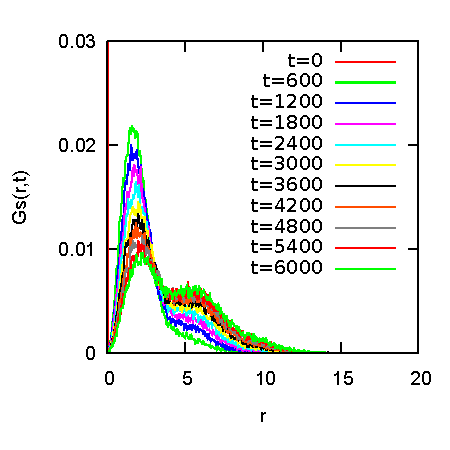
\includegraphics[width=\columnwidth]{Ave_Trj.pdf}

    \centering
    トリブロックコポリマーのクラスタ部に対する $G_s(\bm{r}, t)$ の例
\end{columns}

\end{frame}
%%%%%%%%%%%


\end{document}
